
\section{一条道路的\trMaslovIndex}
\label{sec:maslov-index-path}

\subsection{\trMaslovIndex{}的定义}
\label{subsec:maslov-index-definition}

设 $W^{+}$ 与 $W^{-}$ 分别是 $\mathrm{Sp}(2n)^{+}$ 与 $\mathrm{Sp}(2n)^{-}$ 中取定的两个矩阵，\footnote{译注：原书行文听任 $W^{\pm}$ 任取（“例如……”）；然此处的取法并不能任意，否则下文的\trMaslovIndex{}将失去整数性（\cref{thm:maslov-index-integer}）：例如 $n=1$ 时取 $W^{+}=R(\pi/2)\in\mathrm{Sp}(2)^{+}$（$\det(R(\pi/2)-\mathrm{Id})=2>0$），则 $\rho(W^{+})=e^{i\pi/2}\neq\pm1$，按同一公式对常值道路即得 $\mu=-1/2$，非整数。故应固定使用此处所展示的两个标准矩阵（$\rho(W^{+})=(-1)^{n}$、$\rho(W^{-})=(-1)^{n-1}$），整数性与符号公式皆系于此。此处照原书排印，存疑备案。——译者注}例如上一节的各证明中所用过的那两个，即
\[
W^{+}=-\mathrm{Id}\text{，}\qquad
W^{-}=\left(\begin{array}{cc|c}
2 & 0 & \\
0 & 1/2 & 0\\
\hline
\multicolumn{2}{c|}{0} & -\mathrm{Id}
\end{array}\right)\text{。}
\]

对每条道路 $\gamma\colon[0,1]\longrightarrow\mathrm{Sp}(2n)$，我们选取 $\rho\circ\gamma$ 的一个\trLift{} $\alpha\colon[0,1]\longrightarrow\RR$，
\[
\begin{tikzcd}[column sep=1.5cm,row sep=1.8em]
&& \RR \ar[d,"\exp"'] \\
{[0,1]} \ar[urr,"\alpha"] \ar[r,"\gamma"'] & \mathrm{Sp}(2n) \ar[r,"\rho"'] & S^1
\end{tikzcd}
\]
并令
\[
\Delta(\gamma)=\frac{\alpha(0)-\alpha(1)}{\pi}\text{。}
\]

若 $A\in\mathrm{Sp}(2n)^\star$，我们就选取一条（在 $\mathrm{Sp}(2n)^\star$ 中的）道路 $\gamma_A$，把 $A$ 连到 $\mathrm{Sp}(2n)^{\pm}$ 中的矩阵 $W^{\pm}$。根据\cref{thm:sp-star-components}，$\gamma_A$ 的\trHomotopy{}类是\trWellDefined{}的，特别地，$\Delta(\gamma_A)$ 只依赖于 $A$。于是我们令 $r(A)=\Delta(\gamma_A)$。

\begin{figure}[htbp]
\centering
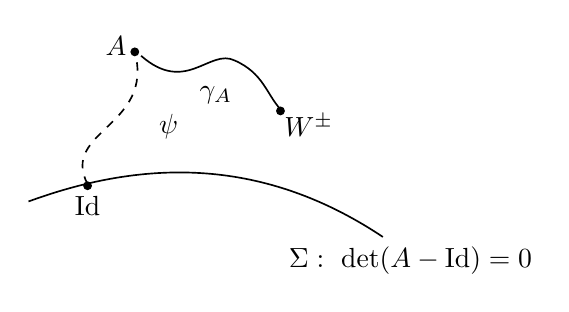
\begin{tikzpicture}[line width=0.6pt]
  \draw (0,0.05) .. controls (1.5,0.6) and (3.0,0.6) .. (4.5,-0.4);
  \node at (4.85,-0.7) {$\Sigma:\ \det(A-\mathrm{Id})=0$};
  \fill (0.75,0.25) circle (1.6pt);
  \node at (0.75,0.0) {$\mathrm{Id}$};
  \draw[dashed] (0.75,0.27) .. controls (0.4,0.95) and (1.6,1.0) .. (1.35,1.95);
  \node at (1.78,1.0) {$\psi$};
  \fill (1.35,1.95) circle (1.6pt);
  \node at (1.11,2.02) {$A$};
  \draw (1.43,1.9) .. controls (2.0,1.4) and (2.3,2.0) .. (2.62,1.84)
        .. controls (2.98,1.68) and (3.02,1.42) .. (3.2,1.22);
  \node at (2.38,1.4) {$\gamma_A$};
  \fill (3.2,1.2) circle (1.6pt);
  \node at (3.56,1.02) {$W^{\pm}$};
\end{tikzpicture}
\caption{}
\label{fig:maslov-path-lift}
\end{figure}

设 $\psi$ 是一条把 $\mathrm{Id}$ 连到 $\mathrm{Sp}(2n)^\star$ 中一个元素的道路。我们如下定义这条道路的\trMaslovIndex{} $\mu(\psi)$：
\[
\mu(\psi)=\Delta(\psi)+r(\psi(1))\text{。}
\]
它就是由 $\psi$ 与 $\gamma_A$ 复合而成的道路在 $\rho$ 之下的像沿\trCircle{}所转出的顺时针“半转”的数目。

\begin{proposition}\label{thm:maslov-index-integer}
\trMaslovIndex{}是一个整数。两条道路 $\psi_0$ 与 $\psi_1$ \trHomotopic{}（端点在 $\mathrm{Sp}(2n)^\star$ 中），当且仅当它们具有相同的\trIndex。此外，我们有：
\begin{itemize}
\item $\det(\psi(1)-\mathrm{Id})$ 的符号是 $(-1)^{\mu(\psi)-n}$。
\item 若 $S$ 是范数 $\|S\|<2\pi$ 的\trInvertible\trSymmetricMatrix，且 $\psi(t)=\exp(tJ_0S)$，则
\[
\mu(\psi)=\operatorname{Ind}(S)-n\text{，}
\]
其中 $\operatorname{Ind}(S)$ 表示 $S$ 的负\trEigenvalue{}的个数。
\end{itemize}
\end{proposition}

\begin{proof}
我们先取道路 $\psi$ 与 $\mathrm{Sp}(2n)^\star$ 中一条把 $\psi(1)$ 连到矩阵 $W^{\pm}$ 的道路的复合——这正是\cref{thm:sp-star-components}所容许的。设 $\gamma$ 为复合而成的道路。我们有
\[
\mu(\psi)=\Delta(\gamma)\in\ZZ
\]
因为 $\rho(W^{\pm})=\pm1$。

此外，由同一条命题，两条道路 $\psi_0$ 与 $\psi_1$ \trHomotopic，当且仅当两个扩张 $\gamma_0$ 与 $\gamma_1$ \trHomotopic{}（端点固定）。映射 $\rho$ 在\trFundamentalGroup{}上诱导一个\trIsomorphism，因此这等价于等式 $\Delta(\gamma_0)=\Delta(\gamma_1)$，也就是说，等价于 $\psi_0$ 与 $\psi_1$ 的\trMaslovIndex{}相等。

设 $\psi$ 是一条道路，$\gamma$ 是如上的一个扩张。若 $\psi(1)\in\mathrm{Sp}(2n)^{+}$，也就是说，若 $\det(\psi(1)-\mathrm{Id})>0$，则 $\gamma$ 的端点位于 $W^{+}=-\mathrm{Id}$ 处，从而 $\rho(\gamma(1))=(-1)^n$。此时 $\mu(\psi)-n$ 是偶数。而若 $\det(\psi(1)-\mathrm{Id})<0$，则 $\gamma$ 走到 $W^{-}$，且 $\rho(\gamma(1))=(-1)^{n-1}$，于是 $\mu(\psi)-n$ 是奇数。

我们还须证明关于\trSymmetricMatrix{}的那条陈述。人们易于验证（\cref{ex:ch14-015-exp-symplectic}）：若 $S$ 是对称的，则 $\exp(tJ_0S)$ 是\trSymplectic{}的。接着，由于 $S$ 是对称的，它在某组\trOrthonormal{}基下\trDiagonalizable，并且存在一条由 $\mathrm{O}^{+}(2n)$ 中矩阵构成的道路 $\lambda\mapsto P(\lambda)$，使得 $P(0)=\mathrm{Id}$ 且 $S(1)={}^tP(1)SP(1)$ 是一个对角矩阵。\footnote{译注：原书此处印作“$\psi_\lambda(t)=\exp(tJS_0(\lambda))$”；疑应为 $\exp(tJ_0S(\lambda))$（$S_0(\lambda)$ 全书无定义，且紧随本句的正文即用 $\exp(J_0S(\lambda))$），系下标 $0$ 误置，此处径改。——译者注}令
\[
S(\lambda)={}^tP(\lambda)SP(\lambda)\qquad\text{以及}\qquad \psi_\lambda(t)=\exp(tJ_0S(\lambda))\text{。}
\]
\trSymmetricMatrix{} $S_\lambda$ 的\trIndex{}（就\trQuadraticForm{}的意义而言）不依赖于 $\lambda$。$S$ 的范数小于 $2\pi$ 这一事实保证 $\exp(J_0S(\lambda))$ 不具有\trEigenvalue{} $1$。于是，对任意的 $\lambda$，我们都能计算道路 $\psi_\lambda$ 的\trMaslovIndex{}（因为这个\trIndex{}不依赖于它，并且 $\psi_\lambda\in\scr{S}$），从而我们就把问题化归为：在\trSymmetricMatrix{}恰好是对角矩阵的情形下证明所要的等式。用同一个论证，我们可以、而且也确实进一步假设 $S$ 的\trEigenvalue{}为 $\pi$ 与 $-\pi$。然后我们把 $\RR^{2n}$ 分解成 $n$ 个\trSymplectic{}平面之和，于是只须对诸\trSymmetricMatrix
\[
\begin{pmatrix}\pi&0\\0&\pi\end{pmatrix}\text{，}\qquad
\begin{pmatrix}\pi&0\\0&-\pi\end{pmatrix}\text{，}\qquad
\begin{pmatrix}-\pi&0\\0&-\pi\end{pmatrix}\text{。}
\]
算出\trMaslovIndex{}即可。的确，\cref{thm:rho-map-properties}中 $\rho$ 的乘性正好转化为\trMaslovIndex{}的可加性。

对第一个矩阵，
\[
\exp(tJ_0S)=\begin{pmatrix}\cos\pi t&-\sin\pi t\\ \sin\pi t&\cos\pi t\end{pmatrix}
\]
是一个转角为 $t\pi$ 的旋转。这个矩阵就是\trUnitary{}矩阵 $\exp(it\pi)$，从而它在 $\rho$ 之下的像是 $\exp(it\pi)$。这就给出了\trMaslovIndex
\[
\mu(\exp(tJ_0S))=-1\ (= \operatorname{Ind}(S)-1)\text{。}
\]

对第三个矩阵做同样的计算，给出
\[
\exp(tJ_0S)=\begin{pmatrix}\cos\pi t&\sin\pi t\\ -\sin\pi t&\cos\pi t\end{pmatrix}\text{，}
\]
这次是一个转角为 $-t\pi$ 的旋转，从而它在 $\rho$ 之下的像是 $\exp(-it\pi)$。这就给出了\trMaslovIndex
\[
\mu(\exp(tJ_0S))=1\ (= \operatorname{Ind}(S)-1)\text{。}
\]

第二个\trSymmetricMatrix{}则给出
\[
\exp(tJ_0S)=\begin{pmatrix}\cosh\pi t&\sinh\pi t\\ \sinh\pi t&\cosh\pi t\end{pmatrix}\text{，}
\]
这是一个\trEigenvalue{}为 $e^{\pi t}$ 与 $e^{-\pi t}$ 的矩阵——两个正实数，于是 $\rho$ 把这个矩阵送到 $1$，且
\[
\mu(\exp(tJ_0S))=0\ (= \operatorname{Ind}(S)-1)\text{。}
\]

于是，对这三种情形我们都有了所述的公式（取 $n=1$），从而由可加性，在一般的情形亦然。
\end{proof}

\subsection{总结：第三步}
\label{subsec:summary-third-step}

在\cref{thm:symplectic-trivialization}之下，我们至此便对每条\trNondegenerate{}且\trContractible{}的、\trPeriodic{}为 $1$ 的\trTrajectory{}都赋予了一个整数，即它的\emph{\trMaslovIndex}。

上面就诸\trSymmetricMatrix{}所做的\trMaslovIndex{}计算，在\trAutonomous{}\trHamiltonian{}量与\trStationary\trTrajectory{}的情形下给出下面的结果。

\begin{corollary}\label{thm:maslov-index-autonomous}
设 $W$ 是一个维数为 $2n$ 的\trSymplectic\trManifold，而
\[
H\colon W\longrightarrow\RR
\]
是一个（\trAutonomous{}的）\trHamiltonian{}量，又设 $x$ 是 $H$ 的一个\trCriticalPoint。我们假设 $H$ 就 $\cC^2$ \trTopology{}而言是小的；此时 $\|\operatorname{Hess}_x(H)\|<2\pi$。那么，$x$ 作为\trHamiltonian{}系统的\trPeriodic{}解的\trMaslovIndex{} $\mu(x)$，与它作为函数 $H$ 的\trCriticalPoint{}的\trIndex{} $\operatorname{Ind}(x)$，由下式联系起来：
\[
\mu(x)=\operatorname{Ind}(x)-n\text{。}
\]
\noqed
\end{corollary}

\subsection{\trSymplectic{}矩阵与\trSymmetricMatrix{}之间的联系}
\label{subsec:symplectic-symmetric-link}

我们知道（由\cref{ex:ch14-015-exp-symplectic}与\cref{thm:maslov-index-integer}），当 $S$ 是一个\trSymmetricMatrix{}时，$\exp(tJ_0S)$ 是一个\trSymplectic{}矩阵。更一般地，我们有下面的结果。

\begin{lemma}\label{thm:symplectic-symmetric-paths}
设 $S\colon[0,1]\longrightarrow M(2n;\RR)$ 是一条由\trSymmetricMatrix{}构成的道路。那么，作为
\[
\frac{d}{dt}R(t)=J_0S(t)R(t)\text{，}\qquad R(0)=\mathrm{Id}
\]
之解的道路 $R\colon[0,1]\longrightarrow M(2n;\RR)$ 属于 $\mathrm{Sp}(2n)$。反之，若 $R\colon[0,1]\longrightarrow\mathrm{Sp}(2n)$ 是一条 $\cC^1$ 类的道路，则道路
\[
S(t)=-J_0R'(t)R(t)^{-1}
\]
由\trSymmetricMatrix{}构成。
\end{lemma}

\begin{proof}
我们以 $'$ 表示对 $t$ 的求导。首先有
\[
{}^tR(t)'=-{}^tR(t)S(t)J_0\text{，}
\]
继而
\[
\begin{aligned}
\bigl({}^tRJ_0R\bigr)'&={}^tR'J_0R+{}^tRJ_0R'\\
&=-{}^tRSJ_0^2R+{}^tRJ_0^2SR\\
&={}^tRSR-{}^tRSR=0\text{，}
\end{aligned}
\]
这表明，对每个 $t\in[0,1]$ 都有 ${}^tRJ_0R=J_0$，从而 $R(t)\in\mathrm{Sp}(2n)$。

反之，我们有另一个计算：\footnote{译注：原书下式末行印作“$R'R^{-1}+RR'^{-1}=0$”；疑应为“$R'R^{-1}+R\bigl(R^{-1}\bigr)'=0$”（由 $\frac{d}{dt}\bigl(RR^{-1}\bigr)=\frac{d}{dt}\,\mathrm{Id}=0$ 展开唯有后式成立），系撇号误置，此处径改。——译者注}
\[
\begin{aligned}
{}^tS&=-{}^t\bigl(J_0R'R^{-1}\bigr)=-{}^tR^{-1}\,{}^tR'\,{}^tJ_0\\
&={}^tR^{-1}\,{}^tR'J_0 &&\text{因为 }J_0\text{ 是}\text{\trAntisymmetric{}}\text{的}\\
&={}^tR^{-1}\bigl({}^tRJ_0\bigr)'\\
&={}^tR^{-1}\bigl(J_0R^{-1}\bigr)' &&\text{因为 }{}^tRJ_0R=J_0\Rightarrow{}^tRJ_0=J_0R^{-1}\\
&={}^tR^{-1}J_0\bigl(R^{-1}\bigr)'\\
&=J_0R\bigl(R^{-1}\bigr)' &&\text{因为，同理，}{}^tR^{-1}J_0=J_0R\\
&=-J_0R'R^{-1} &&\text{因为 }RR^{-1}=\mathrm{Id}\Rightarrow R'R^{-1}+R\bigl(R^{-1}\bigr)'=0\\
&=S\text{。}
\end{aligned}
\]
\end{proof}

\subsection{具有指定\trMaslovIndex{}的道路}
\label{subsec:prescribed-maslov-index}

\begin{lemma}\label{thm:prescribed-maslov-index}
对每个 $k\in\ZZ$，都存在一个对角矩阵 $S_k\in M(2n;\RR)$，使得相伴的道路 $R(t)=\exp(tJ_0S_k)$ 属于 $\scr{S}$ 且满足
\[
\mu(R(t))=k\text{。}
\]
\end{lemma}

\begin{proof}
我们先来推广一个前文已在维数 $2$ 的情形做过的计算。我们选取一个奇整数 $\ell$，并考虑对角矩阵 $S=\begin{pmatrix}\ell\pi&0\\0&\ell\pi\end{pmatrix}$。那么
\[
e^{tJ_0S}=\begin{pmatrix}\cos\ell\pi t&-\sin\ell\pi t\\ \sin\ell\pi t&\cos\ell\pi t\end{pmatrix}
\]
是 $\scr{S}$ 中一条终于 $-\mathrm{Id}=W^{+}\in\mathrm{Sp}(2)^{+}$ 的道路。矩阵 $e^{tJ_0S}$ 就是\trUnitary{}矩阵 $e^{i\ell\pi t}\in\mathrm{U}(1)\subset\mathrm{Sp}(2)$，\footnote{译注：原书此处印作 $e^{i\ell t}$；按 $S=\begin{pmatrix}\ell\pi&0\\0&\ell\pi\end{pmatrix}$，$e^{tJ_0S}$ 作为 $\mathrm{U}(1)$ 中的矩阵应为 $e^{i\ell\pi t}$（下文 $\mu(e^{tJ_0S})=-\ell$ 亦唯与此相配），系漏一因子 $\pi$，此处径改。——译者注}于是 $\mu(e^{tJ_0S})=-\ell$。对 $S=\begin{pmatrix}1&0\\0&-1\end{pmatrix}$，我们有
\[
e^{tJ_0S}=\begin{pmatrix}\cosh t&\sinh t\\ \sinh t&\cosh t\end{pmatrix}\text{，}
\]
这是 $\scr{S}$ 中的一条道路，其诸矩阵的\trEigenvalue{} $e^{t}$ 与 $e^{-t}$ 在 $t>0$ 时是相异的正实数，于是 $\mu(e^{tJ_0S})=0$。

在坐标 $p_1,q_1,\dotsc,p_n,q_n$ 之下，考虑对角矩阵
\[
S_k=\left[\begin{array}{ccccc}
\begin{bmatrix}-\pi&0\\0&-\pi\end{bmatrix}&&&&\\
&\ddots&&&\\
&&\begin{bmatrix}-\pi&0\\0&-\pi\end{bmatrix}&&\\
&&&\begin{bmatrix}-\pi&0\\0&-\pi\end{bmatrix}&\\
&&&&\begin{bmatrix}(n-k-1)\pi&0\\0&(n-k-1)\pi\end{bmatrix}
\end{array}\right]
\]
（若 $k\equiv n\ \mathrm{mod}\ 2$），以及
\[
S_k=\left[\begin{array}{ccccc}
\begin{bmatrix}-\pi&0\\0&-\pi\end{bmatrix}&&&&\\
&\ddots&&&\\
&&\begin{bmatrix}-\pi&0\\0&-\pi\end{bmatrix}&&\\
&&&\begin{bmatrix}1&0\\0&-1\end{bmatrix}&\\
&&&&\begin{bmatrix}(n-k-2)\pi&0\\0&(n-k-2)\pi\end{bmatrix}
\end{array}\right]
\]
（若 $k\equiv n-1\ \mathrm{mod}\ 2$）。\footnote{译注：此处的分块构造默认 $n\geq2$：第二个矩阵除 $\bigl[\begin{smallmatrix}(n-k-2)\pi&0\\0&(n-k-2)\pi\end{smallmatrix}\bigr]$ 分块外还含一枚 $\bigl[\begin{smallmatrix}1&0\\0&-1\end{smallmatrix}\bigr]$ 分块，至少要占两个辛平面，$n=1$ 时排不出来；$n=1$ 时本引理仅能实现 $k=0$（经上文 $S=\begin{pmatrix}1&0\\0&-1\end{pmatrix}$ 的道路）与奇数 $k$（此时第一个矩阵只含单枚 $\bigl[\begin{smallmatrix}-k\pi&0\\0&-k\pi\end{smallmatrix}\bigr]$ 分块，即 $S=\begin{pmatrix}-k\pi&0\\0&-k\pi\end{pmatrix}$）。此处照原书排印，存疑备案。——译者注}由\trMaslovIndex{}的可加性，这些矩阵定义了\trMaslovIndex{}为 $k$ 的道路。
\end{proof}

\begin{remark}\label{thm:maslov-blocks-epsilon}
如果把上述矩阵中前 $n-1$ 个对角分块按下列方式之一替换：
\begin{itemize}
\item 把 $\begin{bmatrix}-\pi&0\\0&-\pi\end{bmatrix}$ 换成 $\begin{bmatrix}-\pi\varepsilon&0\\0&-\pi\varepsilon\end{bmatrix}$；
\item 把 $\begin{bmatrix}1&0\\0&-1\end{bmatrix}$ 换成 $\begin{bmatrix}\varepsilon&0\\0&-\varepsilon\end{bmatrix}$，
\end{itemize}
其中 $\varepsilon>0$ 充分小，那么它们的\trMaslovIndex{}保持不变：用来计算\trMaslovIndex{}的那些介于 $\mathrm{Id}$ 与 $W^{\pm}$ 之间的道路是相同的。
\end{remark}

在第 8 章中，我们将再次使用这些矩阵 $S_k$，并仍用这套记号（不过有时会像\cref{thm:maslov-blocks-epsilon}中那样改动分块）。
